\documentclass[10pt]{article}
\usepackage[polish]{babel}
\usepackage[utf8]{inputenc}
\usepackage[T1]{fontenc}
\usepackage{amsmath}
\usepackage{amsfonts}
\usepackage{amssymb}
\usepackage[version=4]{mhchem}
\usepackage{stmaryrd}
\usepackage{graphicx}
\usepackage[export]{adjustbox}
\graphicspath{ {./images/} }

\title{GIMNAZJUM }

\author{}
\date{}


\begin{document}
\maketitle
\begin{enumerate}
  \item Danych jest w przestrzeni n punktów, z których żadne cztery nie leżą w jednej płaszczyźnie. Każdy z nich łączymy ze wszystkimi pozostałymi używając odcinków w dwóch kolorach. Jaka jest minimalna liczba \(n\), taka że nie można przy tym uniknąć utworzenia się trójkąta o wszystkich bokach jednakowego koloru?
  \item Na rysunku tej figury podano powierzchnię czterech trójkątów. Ile wynosi powierzchnia piątego trójkąta?\\
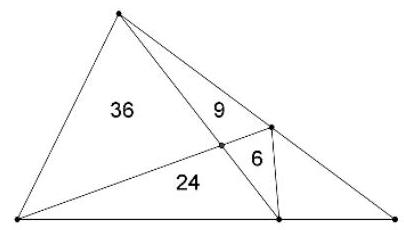
\includegraphics[max width=\textwidth, center]{2024_11_21_2e37a55644ead6a2a668g-1}
  \item Wiedząc, że \(x>0\) i \(x^{2}+\frac{1}{x^{2}}=7\) oblicz \(x^{5}+\frac{1}{x^{5}}\)
\end{enumerate}

\section*{LICEUM}
\begin{enumerate}
  \item Stefania i Tomasz stoją na średnicy okrągłego placu i dzielą tę średnicę na trzy równe części. Po obrzeżu tego placu biega pies przytrzymywany na dwóch elastycznych smyczach. W pewnym momencie pies znajduje się w punkcie C oraz odległość CS wynosi 7 m , a odległość CT wynosi 9 m. Jaka jest odległość między Stefanią i Tomaszem?
  \item Funkcja \(f\), określona na zbiorze wszystkich dodatnich liczb rzeczywistych i przyjmująca wartości rzeczywiste, spełnia dla każdego \(x>0\) warunek \(2 f(x)+3 f\left(\frac{2017}{x}\right)=5 x\). Oblicz \(f(3)\).
  \item Dany jest trójkąt prostokątny o przyprostokątnych długości odpowiednio \(a\) i \(b\). Na pierwszej z tych przyprostokątnych wybrano punkt \(P\), a na drugiej punkt \(Q\). Niech \(K\) i \(H\) będą rzutami prostokątnymi odpowiednio punktów \(P\) i \(Q\) na przeciwprostokątną. Jaka jest najmniejsza możliwa wartość sumy \(|K P|+|P Q|+|Q H|\) ? Odpowiedź uzasadnij.
\end{enumerate}

\end{document}